\documentclass[slidestop]{beamer}

\title{Project planning}
\providecommand{\myConference}{NBIC BioAssist meeting}
\providecommand{\myDate}{Friday, 20 May 2011}
\author{Jeroen F. J. Laros}
\providecommand{\myGroup}{Leiden Genome Technology Center}
\providecommand{\myDepartment}{Department of Human Genetics}
\providecommand{\myCenter}{Center for Human and Clinical Genetics}
\providecommand{\lastCenterLogo}{
  \raisebox{-0.1cm}{
    \includegraphics[scale = 0.055]{lgtc_logo}
  }
}
\providecommand{\lastRightLogo}{
  \includegraphics[scale = 0.1]{nbic_logo} 
}

\usetheme{lumc}

../Presentation_24-02-11_HumGen_Mutalyzer2/lstBNF.tex
\providecommand{\positionpicture}{
  \vspace{-0.5cm}
  \begin{center}
    \fbox{
      \begin{picture}(300, 60)(0, 0)
        \put(0, 30){\line(1, 0){300}}  % Genomic sequence.
        \linethickness{4pt}
        \put(50, 30){\line(1, 0){30}}  % Non-coding parts of the exons.
        \put(220, 30){\line(1, 0){10}}
        \linethickness{12pt}
        \put(80, 30){\line(1, 0){20}}  % Coding parts of the exons.
        \put(150, 30){\line(1, 0){20}}
        \put(200, 30){\line(1, 0){20}}

        \linethickness{0.5pt}
        \put(20, 50){\scriptsize{Transcription start}}
        \put(50, 45){\vector(0, -1){10}}
        \put(200, 50){\scriptsize{Transcription end}}
        \put(230, 45){\vector(0, -1){10}}

        \put(70, 0){\scriptsize{CDS start}}
        \put(80, 10){\vector(0, 1){10}}
        \put(210, 0){\scriptsize{CDS stop}}
        \put(220, 10){\vector(0, 1){10}}

        \put(0, 0){\scriptsize{Genomic end}}
        \put(0, 10){\vector(0, 1){10}}
        \put(255, 0){\scriptsize{Genomic start}}
        \put(300, 10){\vector(0, 1){10}}

        \put(95, 50){\color{yellow}\scriptsize{Variant A}\color{white}}
        \put(115, 45){\color{yellow}\vector(0, -1){10}\color{white}}

        \put(140, 50){\color{yellow}\scriptsize{Variant B}\color{white}}
        \put(160, 45){\color{yellow}\vector(0, -1){10}\color{white}}
      \end{picture}
    }
  \end{center}
  \bigskip
}

\setlength{\unitlength}{1pt}

\begin{document}

% This disables the \pause command, handy in the editing phase.
%\renewcommand{\pause}{}

% Make the title page.
\bodytemplate

% First page of the presentation.
\section{Introduction}
\begin{frame}
  Common approaches:
  \begin{itemize}
    \item Just start.
    \item Make sure the simple things work, the rest comes later.
  \end{itemize}
  \bigskip
  \pause

  However, it is likely that:
  \begin{itemize}
    \item Specific cases are solved, not parts of the problem.
    \item Unscalable solution are made.
    \item Unmaintainable solution are made.
    \item Lots of time is spent on rewriting.
    \begin{itemize}
      \item Or worse, a stack of exceptions is made.
    \end{itemize}
    \item More time than needed is wasted.
  \end{itemize}
  \bigskip
  \pause

  Software needs to be \emph{designed}.
\end{frame}

\begin{frame}
  Mutalyzer: a curational tool for \emph{Locus Specific Mutation Databases}
  (LSDBs).

  \bigskip
  \begin{itemize}
    \pause
    \item Variant nomenclature checker applying \emph{Human Genome Variation
          Society} (HGVS) guidelines.
    \begin{itemize}
      \item Is the syntax of the variant description valid?
      \item Does the reference sequence exist?
      \item Is the variant possible on this reference sequence?
      \item Is this variant description the recommended one?
    \end{itemize}
    \pause
    \item Basic effect prediction.
    \begin{itemize}
      \item Is the description of the transcript product as expected?
      \item Is the predicted protein as expected?
    \end{itemize}
  \end{itemize}
\end{frame}

\section{HGVS nomenclature}
\begin{frame}
  \emph{Genomic} orientated positions:
  \begin{center}
    \bt{AL449423.14:g.[65449\_65463del;65564\color{yellow}T\color{white}>\color{yellow}C\color{white}]}
  \end{center}
  \pause
  \bigskip
  \emph{Coding sequence} orientated positions:
  \begin{center}
    \bt{AL449423.14(CDKN2A\_v001):c.[5\color{yellow}A\color{white}>\color{yellow}G\color{white}
      ;106\_120del]}
  \end{center}
  \bigskip
  \pause
  \begin{itemize}
    \item \bt{AL449423.14} -- reference sequence.
    \item \bt{CDKN2A\_v001}$\;$ -- transcript variant \bt{1} of gene CDKN2A.
    \item \bt{c.[5\color{yellow}A\color{white}>\color{yellow}G\color{white};106\_120del]}
    \begin{itemize}
      \item A \emph{substitution} at position \bt{5} counting from the start
        codon.
      \item A \emph{deletion} from position \bt{106} to position \bt{120}.
    \end{itemize}
  \end{itemize}
\end{frame}

\begin{frame}
  \positionpicture

  \renewcommand{\arraystretch}{1}
  \begin{center}
    \begin{tabular}{l|r|r|r}
      Name                              & \bt{g.}  & \bt{n.}      & \bt{c.} \\
      \hline
      {\scriptsize Genomic start}       & \bt{1}   & \bt{100+d70} &
        \bt{*10+d70} \\
      {\scriptsize Genomic end}         & \bt{300} & \bt{1-u50}   &
        \bt{-30-u50} \\
      {\scriptsize Transcription start} & \bt{250} & \bt{1}       & \bt{-30} \\
      {\scriptsize Transcription end}   & \bt{70}  & \bt{100}     & \bt{*10} \\
      {\scriptsize CDS start}           & \bt{220} & \bt{30}      & \bt{1} \\
      {\scriptsize CDS stop}            & \bt{80}  & \bt{90}      & \bt{60} \\
    \end{tabular}
  \end{center}
\end{frame}

\begin{frame}
  \positionpicture

  \bt{c.} positions:
  \bigskip
  \begin{itemize}
    \item Positions in introns are relative to the nearest exonic position.
    \item Positions before the CDS are indicated with a \bt{-} sign.
    \item Positions after the CDS are indicated with a \bt{*} sign.
  \end{itemize}

  \pause
  \bigskip
  Position \bt{-1} and \bt{1} are adjacent.

  If \bt{60} is the last position of the CDS, then \bt{60} and \bt{*1} are
  adjacent.
\end{frame}

\section{Mutalyzer 1.0.4}
\begin{frame}
  Organic growth:
  \begin{itemize}
    \item Developed in over four years by multiple people.
    \item Originally a command line program.
    \item Web interface added later.
    \begin{itemize}
      \item PHP scripts that call (exec) a python program.
    \end{itemize}
  \end{itemize}
  \bigskip
  \pause

  Design flaws:
  \begin{itemize}
    \item Nomenclature rules interwoven with the code.
    \item HTML output interwoven with the code.
    \item No modularity (reuse of code is very hard).
    \item Reference sequence parsing not abstracted 
    \begin{itemize}
      \item Support for other reference sequences nearly impossible.
    \end{itemize}
    \item Nomenclature was not analysed / formalised.
    \begin{itemize}
      \item Regular expressions directly in code.
      \item Virtually impossible to change (or read).
    \end{itemize}
  \end{itemize}
\end{frame}

\begin{frame}
  Implementation flaws:
  \begin{itemize}
    \item Inheritance of types (delins on DNA $\Rightarrow$ delins on protein).
    \item Disambiguation not general.
    \item No support of up- / downstream exons.
    \item Nothing was ever redesigned, only wrapped in loops.
    \begin{itemize}
      \item Debugging, altering code made impossible.
      \item Speed drastically diminished.
    \end{itemize}
  \end{itemize}
  \bigskip
  \pause

  Programming flaws:
  \begin{itemize}
    \item Excessive usage of exceptions.
    \item Incomprehensible error messages.
    \item Virtually no inline comment.
    \item Non existent documentation (apart from the user manual).
  \end{itemize}
\end{frame}

\begin{frame}
  Feature requests:
  \begin{itemize}
    \item Solving all mentioned problems.
    \item \color<2>{yellow}{Support for other reference files (LRG).}
    \item \color<2>{yellow}{Programmatic access to internal functions.}
    \item \color<2>{yellow}{Extension of HGVS nomenclature rules.}
  \end{itemize}
  \bigskip
  \pause

  Especially since:
  \begin{itemize}
    \item Interwoven nomenclature.
    \item Interwoven interface.
    \item Lack of documentation.
  \end{itemize}
  \bigskip
  \pause

  Throw away four years of work and start again.
\end{frame}

\section{Preparing for version 2.0}
\begin{frame}
  Preparations for a new version:
  \begin{itemize}
    \item Setting up two version control repositories.
    \item Gathering all old versions and putting then under version control.
    \begin{itemize}
      \item Critical bugfixes until there is a new version.
      \item Easy to search and track changes.
      \item Point of reference for the new version.
    \end{itemize}
    \item Set up bugtracking systems.
    \pause
    \item Talking for months.
    \begin{itemize}
      \item Figuring out what the HGVS language is.
      \item Formalising that language (BNF).
      \item Semantic rules.
    \end{itemize}
    \item Identify and implement functional modules.
    \item Designing interfaces (web (TAL), webservice, command line, \ldots).
    \item Documentation (API (epydoc), TRM, User manual, \ldots).
  \end{itemize}
\end{frame}

\begin{frame}
  Although the complexity might seem low at first glance\ldots
  \bigskip
  
  Non-trivial problems can be found:
  \begin{itemize}
    \item Position systems.
    \begin{itemize}
      \item Reference sequence related peculiarities.
    \end{itemize}
    \item \only<2>{\color{yellow}}The HGVS nomenclature.\only<2>{\color{white}}
    \item Parsing reference sequence files and their annotation.
    \begin{itemize}
      \item Keeping the option open for other formats (LRG).
    \end{itemize}
    \item Keeping track of positions after mutation.
    \item \ldots
  \end{itemize}
\end{frame}

\section{HGVS parser}
\begin{frame}
  The previous versions used \emph{regular expressions} for input parsing.
  \begin{itemize}
    \item The HGVS nomenclature turns out to be a \emph{context free} language.
    \begin{itemize}
      \item Strictly stronger than regular language.
      \item Can not be parsed with a finite automaton.
      \item No regular expressions.
    \end{itemize}
    \item The semantics of the HGVS is even more complex than the syntax.
  \end{itemize}
  \bigskip
  \pause

  These observations remind us of \emph{compiler construction}.
  \begin{itemize}
    \item We need a context free parser.
    \item A parse tree must be generated.
    \item And then there is the semantic checking.
    \begin{itemize}
      \item This should be the real focus of the project, the rest can be
        solved with existing techniques.
    \end{itemize}
  \end{itemize}
\end{frame}

\begin{frame}[fragile]
  Definition of a gene symbol.
  \begin{lstlisting}[language = BNF, caption = {Abstract HGVS nomenclature}]
    TransVar   -> `_v' Number
    ProtIso    -> `_i' Number
    GeneSymbol -> `(' Name (TransVar | ProtIso)? `)'
  \end{lstlisting}

  Gene name and optionally a transcript or isoform number.
  \bigskip
  \bigskip
  \bigskip
  \pause

  \begin{lstlisting}[caption = {HGVS nomenclature in Python}]
      TransVar = Suppress("_v") + Number("TransVar")
      ProtIso = Suppress("_i") + Number("ProtIso")
      GeneSymbol = Suppress('(') + \
          Group(Name("GeneSymbol") + \
          Optional(TransVar ^ ProtIso))("Gene") + \
          Suppress(')')
  \end{lstlisting}
\end{frame}

\begin{frame}[fragile]
  After parsing, a nested python object (parse tree) is generated:
  \bigskip
  \pause

  The generated object of \bt{(CDKN2A\_v001)}:
  \begin{lstlisting}[caption = {Python object}]
      Gene.GeneSymbol = CDKN2A
      Gene.TransVar = 001
  \end{lstlisting}
  \bigskip
  \pause

  Complete BNF consists of $63$ production rules.
  \bigskip
  \medskip
  \pause

  \emph{
    A formalized description of the standard human variant nomenclature will
    improve sequence variant recognition in databases and literature.
  }
  \vspace{0.1cm}

  \scriptsize{
    Jeroen F. J. Laros$^1$, Andr\'e Blavier$^2$, Johan T. den Dunnen$^1$,
    Peter E. M. Taschner$^1$
  }
  \vspace{0.1cm}

  \tiny{
    $^1$ Department of Human Genetics, Center for Human and Clinical Genetics,
    Leiden University Medical Center, Leiden, Nederland
    \vspace{-0.2cm}

    $^2$ Interactive Biosoftware, Rouen, France
  }
\end{frame}

\section{Interfaces}
\begin{frame}
  
  \begin{tabular}{l@{\ \ -\ \ }l}
    Name checker       & Full nomenclature / semantic check.\\
    Syntax checker     & Only nomenclature check.\\
    Position converter & Mapping, lifting over (build / transcripts).\\
    SNP converter      & DbSNP rsId to HGVS.\\
    Name generator     & Point and click to make a description.\\
    GenBank Uploader   & Custom reference sequences.
  \end{tabular}
  \pause
  \bigskip

  Bulk / RPC interfaces:
  \begin{itemize}
    \item Upload a table (CSV, Excel, Open Office Spreadsheet):
    \begin{itemize}
      \item Name checker.
      \item Name checker.
      \item Syntax checker.
      \item Position converter.
      \item SNP converter.
    \end{itemize}
    \item Webservices (SOAP).
    \begin{itemize}
      \item $18$ functions available.
    \end{itemize}
  \end{itemize}
\end{frame}

\section{Components}
\begin{frame}
  \only<2->{\color{gray}}
  \begin{tabular}{l@{\ \ -\ \ }l}
    \color<2,3,4,5,7>{white}{Config}   & Parsing config file.\\
    \color<2,4>{white}{Crossmap}       & Position conversions.\\
    \color<2,4,7>{white}{Db}           & Mapping, linking, queues, caching info.\\
    \color<0,8>{white}{File}           & CSV, Excel, OpenOffice tables.\\
    \color<2,7>{white}{GenRecord}      & Abstraction of annotated reference sequences.\\
    \color<2,7>{white}{GBparser}       & Instance of GenRecord (GenBank files).\\
    \color<2>{white}{LRGparser}        & Instance of GenRecord (LRG files).\\
    \color<2,7>{white}{Misc}           & \\
    \color<2>{white}{Mutator}          & Modify the reference sequence and annotation.\\
    \color<2,3,4,5,6,7>{white}{Output} & Communication with the interfaces.\\
    \color<2,3,4>{white}{Parser}       & HGVS nomenclature parser.\\
    \color<2,5,7>{white}{Retriever}    & Retrieve / cache reference sequences.\\
    \color<8>{white}{Scheduler}        & Batch jobs scheduler.\\
    \color<9>{white}{Serializers}      & SOAP definitions of complex objects.
  \end{tabular}
  \only<2->{\color{white}}

  \begin{center}
    \only<2>{Name checker.}
    \only<3>{Syntax checker.}
    \only<4>{Position converter.}
    \only<5>{SNP converter.}
    \only<6>{Name generator.}
    \only<7>{GenBank Uploader.}
    \only<8>{Added when using a batch interface.}
    \only<9>{Added when using webservices.}
  \end{center}
\end{frame}

\section{Comparison to the old version}
\begin{frame}
  \begin{figure}
    \colorbox{white} {
      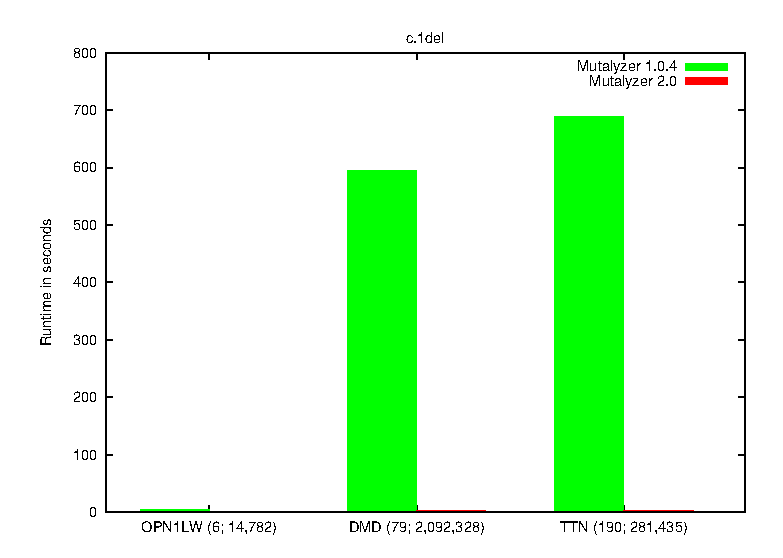
\includegraphics[scale = 0.65]{genes}
    }
    \caption{Runtime comparison}
  \end{figure}
  \vspace{-0.5cm}
  A $229\times$ speedup was measured ($12min$ to $3s$).
\end{frame}

\begin{frame}
  \begin{figure}
    \colorbox{white} {
      \includegraphics[scale = 0.65]{allele}
    }
    \caption{Scalability}
  \end{figure}
  \vspace{-0.5cm}
  Overhead ($\pm 2.5s$): loading the reference sequence.
\end{frame}

\begin{frame}
  Special focus on documentation.

  \begin{table}
    \begin{tabular}{l|l|l}  
                        & 2.0                & 1.0.4 \\
      \hline
      User manual       & $12$ pages         & $12$ pages \\
      TRM               & $31$ pages         & $-$ \\
      API documentation & $215$ pages        & $-$ \\
      Total size        & $493,\!816$ bytes  & $367,\!836$ bytes \\
      Code              & $198,\!512$ bytes  & $245,\!677$ bytes \\
      Comment           & $60\%$             & $33\%^*$ \\
      Development time  & $<1$ year          & $>4$ years
    \end{tabular}
    \caption{Other characteristics.}
  \end{table}

  $^*$ Mostly discarded code.
\end{frame}

\section{Conclusions}
\begin{frame}
  Things to keep in mind:
  \pause
   
  \begin{itemize}
    \item Do not get tempted to implement small exceptions.
    \pause
    \item Make a design.
    \begin{itemize}
      \item Requirements will change in the future.
      \item Make your design capable to deal with these changes.
    \end{itemize}
    \item If requirements change, go back to your design.
    \pause
    \item Document everything.
    \begin{itemize}
      \item Especially your code.
    \end{itemize}
    \pause
    \item Use a version control system.
  \end{itemize}
  \bigskip
  \pause

  Think before you start.
\end{frame}

\section{Questions?}
\lastpagetemplate
\begin{frame}
  \begin{center}
    Acknowledgements:
    \bigskip
    \bigskip

    Martijn Vermaat\\
    Gerben Stouten\\
    Andr\'e Blavier\\
    Gerard Schaafsma\\
    Ivo Fokkema\\
    Jacopo Celli\\
    Peter Taschner\\
    Johan den Dunnen
    \bigskip
    \bigskip
    \bigskip

    \bt{http://www.mutalyzer.nl/}
  \end{center}
\end{frame}

\end{document}
